\scanpage{101}
% archive foliation: 100
\[
\left\{\begin{array}{l}
X=P^2-T'\\
Y=T-T'\\
U=P^2-T
\end{array}\right.
\]

\figure{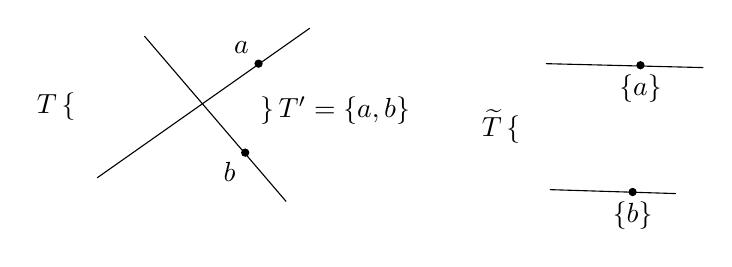
\begin{tikzpicture}[x=1cm,y=1cm]
\draw (0,0)--(2.7,1.9);
\draw (.6,1.8)--(2.4,-.3);
\fill (2.05,1.45) circle (1.5pt) node[above left] {$a$};
\fill (1.88,.32) circle (1.5pt) node[below left] {$b$};
\node at (-.5,.9) {$T\left\{\vphantom{\begin{matrix}a\\a\\a\\a\\a\end{matrix}}\right.$};
\node at (3,.85) {$\left.\vphantom{\begin{matrix}a\\a\\a\end{matrix}}\right\}T'=\{a,b\}$};
\draw (5.7,1.45)--(7.7,1.4);
\draw (5.75,-.15)--(7.35,-.2);
\fill (6.9,1.43) circle (1.5pt) node[below] {$\{a\}$};
\fill (6.8,-.18) circle (1.5pt) node[below] {$\{b\}$};
\node at (5.15,.65) {$\widetilde T\left\{\vphantom{\begin{matrix}a\\a\\a\\a\\a\end{matrix}}\right.$};
\end{tikzpicture}}

\diagram{\begin{tikzcd}
H^1(\widetilde Y)\deleted{\unsure{a}} \arrow[dr] & & \\
H^3_Y(X) \arrow[r] & H^3_{\deleted{\unsure{!}}}(X) \arrow[r,dash] & H^3(U)
\end{tikzcd}}

\diagram{\begin{tikzcd}
H^1_!(Y) & H^1_!(X) \arrow[l] \arrow[dl] & H^1_!(U) \arrow[l] \arrow[d,equal] \\
H^1_!(\widetilde Y) & & 0\quad\text{car }T\text{ connexe}
\end{tikzcd}}

\margin{$H^0($}

\diagram{\begin{tikzcd}
H^0(\widetilde T') \arrow[r] & H^0_{\unsure{!}}(\widetilde T) \arrow[r] & H^1_!(\widetilde Y) \arrow[r,no head] & H^1(\widetilde T') \\
H^0(P^2) \arrow[r] \arrow[u] & H^0(T') \arrow[r] \arrow[u] & H^1_!(X) \arrow[r,no head] \arrow[u] & \substack{H^1(P^2)\\\Vert\\\unsure{0}} \arrow[u] \\
H^0(P^2) \arrow[r] & H^0(T) \arrow[r] \arrow[u] & H^1_!(U) \arrow[r,no head] \arrow[u] & \substack{H^1(P^2)\\\Vert\\\unsure{0}}
\end{tikzcd}}

\margin{$\left\{\begin{array}{l}T\ \uline{connexe}\\T'\ \text{disconnexe},\ \deleted{\text{et}}\\\text{contenu dans }\unsure{\text{l'ou.}}\\\deleted{\text{lieu}}\ \text{de lissité},\\\text{et tte comp. de}\\T'\ \text{contient au}\\\text{plus un}\\\text{point de}\\T'.\end{array}\right.$}

\diagram{\begin{tikzcd}[column sep=large]
& & H^0(T')/\operatorname{Im}H^0(P^2) \arrow[dl,"\text{inj?}"] & H^0(T)/\operatorname{Im}H^0(P^2) \arrow[l] \arrow[d,equal] \\
H^1_!(\widetilde Y) \arrow[r] & H^0(\widetilde T/\operatorname{Im}H^0(\widetilde T') \arrow[dr,equal] & & 0 \\
& & 0 &
\end{tikzcd}}

$\deleted{\unsure{H^1_!}}$

\hrule
